\documentclass[twoside]{book}

% Packages required by doxygen
\usepackage{fixltx2e}
\usepackage{calc}
\usepackage{doxygen}
\usepackage[export]{adjustbox} % also loads graphicx
\usepackage{graphicx}
\usepackage[utf8]{inputenc}
\usepackage{makeidx}
\usepackage{multicol}
\usepackage{multirow}
\PassOptionsToPackage{warn}{textcomp}
\usepackage{textcomp}
\usepackage[nointegrals]{wasysym}
\usepackage[table]{xcolor}

% Font selection
\usepackage[T1]{fontenc}
\usepackage[scaled=.90]{helvet}
\usepackage{courier}
\usepackage{amssymb}
\usepackage{sectsty}
\renewcommand{\familydefault}{\sfdefault}
\allsectionsfont{%
  \fontseries{bc}\selectfont%
  \color{darkgray}%
}
\renewcommand{\DoxyLabelFont}{%
  \fontseries{bc}\selectfont%
  \color{darkgray}%
}
\newcommand{\+}{\discretionary{\mbox{\scriptsize$\hookleftarrow$}}{}{}}

% Page & text layout
\usepackage{geometry}
\geometry{%
  a4paper,%
  top=2.5cm,%
  bottom=2.5cm,%
  left=2.5cm,%
  right=2.5cm%
}
\tolerance=750
\hfuzz=15pt
\hbadness=750
\setlength{\emergencystretch}{15pt}
\setlength{\parindent}{0cm}
\setlength{\parskip}{3ex plus 2ex minus 2ex}
\makeatletter
\renewcommand{\paragraph}{%
  \@startsection{paragraph}{4}{0ex}{-1.0ex}{1.0ex}{%
    \normalfont\normalsize\bfseries\SS@parafont%
  }%
}
\renewcommand{\subparagraph}{%
  \@startsection{subparagraph}{5}{0ex}{-1.0ex}{1.0ex}{%
    \normalfont\normalsize\bfseries\SS@subparafont%
  }%
}
\makeatother

% Headers & footers
\usepackage{fancyhdr}
\pagestyle{fancyplain}
\fancyhead[LE]{\fancyplain{}{\bfseries\thepage}}
\fancyhead[CE]{\fancyplain{}{}}
\fancyhead[RE]{\fancyplain{}{\bfseries\leftmark}}
\fancyhead[LO]{\fancyplain{}{\bfseries\rightmark}}
\fancyhead[CO]{\fancyplain{}{}}
\fancyhead[RO]{\fancyplain{}{\bfseries\thepage}}
\fancyfoot[LE]{\fancyplain{}{}}
\fancyfoot[CE]{\fancyplain{}{}}
\fancyfoot[RE]{\fancyplain{}{\bfseries\scriptsize Generated by Doxygen }}
\fancyfoot[LO]{\fancyplain{}{\bfseries\scriptsize Generated by Doxygen }}
\fancyfoot[CO]{\fancyplain{}{}}
\fancyfoot[RO]{\fancyplain{}{}}
\renewcommand{\footrulewidth}{0.4pt}
\renewcommand{\chaptermark}[1]{%
  \markboth{#1}{}%
}
\renewcommand{\sectionmark}[1]{%
  \markright{\thesection\ #1}%
}

% Indices & bibliography
\usepackage{natbib}
\usepackage[titles]{tocloft}
\setcounter{tocdepth}{3}
\setcounter{secnumdepth}{5}
\makeindex

% Hyperlinks (required, but should be loaded last)
\usepackage{ifpdf}
\ifpdf
  \usepackage[pdftex,pagebackref=true]{hyperref}
\else
  \usepackage[ps2pdf,pagebackref=true]{hyperref}
\fi
\hypersetup{%
  colorlinks=true,%
  linkcolor=blue,%
  citecolor=blue,%
  unicode%
}

% Custom commands
\newcommand{\clearemptydoublepage}{%
  \newpage{\pagestyle{empty}\cleardoublepage}%
}

\usepackage{caption}
\captionsetup{labelsep=space,justification=centering,font={bf},singlelinecheck=off,skip=4pt,position=top}

%===== C O N T E N T S =====

\begin{document}

% Titlepage & ToC
\hypersetup{pageanchor=false,
             bookmarksnumbered=true,
             pdfencoding=unicode
            }
\pagenumbering{alph}
\begin{titlepage}
\vspace*{7cm}
\begin{center}%
{\Large Sof\+AR }\\
\vspace*{1cm}
{\large Generated by Doxygen 1.8.14}\\
\end{center}
\end{titlepage}
\clearemptydoublepage
\pagenumbering{roman}
\tableofcontents
\clearemptydoublepage
\pagenumbering{arabic}
\hypersetup{pageanchor=true}

%--- Begin generated contents ---
\chapter{Class Index}
\section{Class List}
Here are the classes, structs, unions and interfaces with brief descriptions\+:\begin{DoxyCompactList}
\item\contentsline{section}{\hyperlink{classDrone}{Drone} }{\pageref{classDrone}}{}
\item\contentsline{section}{\hyperlink{structPoint}{Point} }{\pageref{structPoint}}{}
\end{DoxyCompactList}

\chapter{File Index}
\section{File List}
Here is a list of all files with brief descriptions\+:\begin{DoxyCompactList}
\item\contentsline{section}{pddl\+\_\+\+Gazebo/include/\hyperlink{pddl__Gazebo_2include_2Drone_8h}{Drone.\+h} }{\pageref{pddl__Gazebo_2include_2Drone_8h}}{}
\item\contentsline{section}{pddl\+\_\+\+Gazebo/lib/\hyperlink{pddl__Gazebo_2lib_2Drone_8cpp}{Drone.\+cpp} }{\pageref{pddl__Gazebo_2lib_2Drone_8cpp}}{}
\item\contentsline{section}{pddl\+\_\+\+Gazebo/src/\hyperlink{pddl__Gazebo_2src_2main_8cpp}{main.\+cpp} }{\pageref{pddl__Gazebo_2src_2main_8cpp}}{}
\item\contentsline{section}{pddl\+\_\+real\+Drones/include/\hyperlink{pddl__realDrones_2include_2Drone_8h}{Drone.\+h} }{\pageref{pddl__realDrones_2include_2Drone_8h}}{}
\item\contentsline{section}{pddl\+\_\+real\+Drones/lib/\hyperlink{pddl__realDrones_2lib_2Drone_8cpp}{Drone.\+cpp} }{\pageref{pddl__realDrones_2lib_2Drone_8cpp}}{}
\item\contentsline{section}{pddl\+\_\+real\+Drones/src/\hyperlink{pddl__realDrones_2src_2main_8cpp}{main.\+cpp} }{\pageref{pddl__realDrones_2src_2main_8cpp}}{}
\item\contentsline{section}{Sof\+A\+R/\hyperlink{build__problem_8c}{build\+\_\+problem.\+c} \\*Script that builds the map and the problem for the pddl plan }{\pageref{build__problem_8c}}{}
\end{DoxyCompactList}

\chapter{Class Documentation}
\hypertarget{classDrone}{}\section{Drone Class Reference}
\label{classDrone}\index{Drone@{Drone}}


{\ttfamily \#include $<$Drone.\+h$>$}

\subsection*{Public Member Functions}
\begin{DoxyCompactItemize}
\item 
\hyperlink{classDrone_ab692baa4be5c43b72990ce1b01bdc805}{Drone} ()
\item 
\hyperlink{classDrone_a667075abb1eb5c54be6418884a387d14}{$\sim$\+Drone} ()
\item 
std\+::string \hyperlink{classDrone_a1fcaf0892001bf12b99c838e64878d9e}{get\+Name} ()
\item 
void \hyperlink{classDrone_a16ee9c16220886633f98e591c9e3dac5}{set\+Current\+Position} (const geometry\+\_\+msgs\+::\+Pose\+Stamped position)
\item 
geometry\+\_\+msgs\+::\+Pose\+Stamped \hyperlink{classDrone_a0113e8f3a3f438113dca0d77c065276b}{get\+Current\+Position} ()
\item 
void \hyperlink{classDrone_a9addfdac3dc0e676ba12c1f4ced68fbe}{set\+Next\+Position} (geometry\+\_\+msgs\+::\+Pose\+Stamped position)
\item 
geometry\+\_\+msgs\+::\+Pose\+Stamped \hyperlink{classDrone_a6a6df41b8eae2b1d6c2b66f046fe5a24}{get\+Next\+Position} ()
\item 
void \hyperlink{classDrone_a8d6917c3191ec7f675b246895ffa6a0d}{set\+Publisher} (ros\+::\+Node\+Handle nh)
\item 
ros\+::\+Publisher \hyperlink{classDrone_aac0983a112b0b3f75c0e625bcba3a330}{get\+Publisher} ()
\item 
bool \hyperlink{classDrone_a106284f63c05f3f112435b2cb5c4896c}{move} (float X, float Y, float Z)
\item 
void \hyperlink{classDrone_a8598b7ea716264e8428a4963a13252fb}{set\+Drone} (int number, std\+::string \hyperlink{classDrone_a19bf0a73d086997ba0589984c58b62da}{path}, ros\+::\+Node\+Handle nh)
\item 
\hyperlink{classDrone_ab692baa4be5c43b72990ce1b01bdc805}{Drone} ()
\item 
\hyperlink{classDrone_a667075abb1eb5c54be6418884a387d14}{$\sim$\+Drone} ()
\item 
std\+::string \hyperlink{classDrone_a1fcaf0892001bf12b99c838e64878d9e}{get\+Name} ()
\item 
void \hyperlink{classDrone_a16ee9c16220886633f98e591c9e3dac5}{set\+Current\+Position} (const geometry\+\_\+msgs\+::\+Pose\+Stamped position)
\item 
geometry\+\_\+msgs\+::\+Pose\+Stamped \hyperlink{classDrone_a0113e8f3a3f438113dca0d77c065276b}{get\+Current\+Position} ()
\item 
void \hyperlink{classDrone_a9addfdac3dc0e676ba12c1f4ced68fbe}{set\+Next\+Position} (geometry\+\_\+msgs\+::\+Pose\+Stamped position)
\item 
geometry\+\_\+msgs\+::\+Pose\+Stamped \hyperlink{classDrone_a6a6df41b8eae2b1d6c2b66f046fe5a24}{get\+Next\+Position} ()
\item 
bool \hyperlink{classDrone_a106284f63c05f3f112435b2cb5c4896c}{move} (float X, float Y, float Z)
\item 
void \hyperlink{classDrone_a2ce35a5df79f379f6f8d3586d444c3f4}{set\+Drone} (int number, ros\+::\+Node\+Handle nh)
\end{DoxyCompactItemize}
\subsection*{Protected Attributes}
\begin{DoxyCompactItemize}
\item 
std\+::string \hyperlink{classDrone_a19bf0a73d086997ba0589984c58b62da}{path}
\item 
std\+::string \hyperlink{classDrone_ac5f6c269378659247acd057142542013}{name}
\item 
geometry\+\_\+msgs\+::\+Pose\+Stamped \hyperlink{classDrone_a190e4f63bb9a0e5b4f822fc87f2185f9}{current\+Position}
\item 
geometry\+\_\+msgs\+::\+Pose\+Stamped \hyperlink{classDrone_a49f95c0480f27c22c122f5bb8482e914}{next\+Position}
\item 
ros\+::\+Publisher \hyperlink{classDrone_a4bdfc664da2ebff40d9a4b413e4ea768}{pub}
\item 
ros\+::\+Subscriber \hyperlink{classDrone_a8baae58c4cbe6f1a8d239fca2d3496d6}{pose\+Sub}
\item 
actionlib\+::\+Simple\+Action\+Client$<$ asctec\+\_\+hl\+\_\+comm\+::\+Waypoint\+Action $>$ $\ast$ \hyperlink{classDrone_a767d339ed35d7be9c8ea4709a8dccb47}{ac}
\item 
float \hyperlink{classDrone_a915ef72b30c96172ff8f295cbb7f47d4}{max\+Speed} =0.\+3
\item 
float \hyperlink{classDrone_afbbc1d4b668c6d5021344f0578c12973}{accuracy} =0.\+3
\end{DoxyCompactItemize}


\subsection{Detailed Description}
\begin{DoxyAuthor}{Authors}
B\+O\+R\+E\+L\+LO -\/ B\+R\+A\+S\+S\+E\+UR
\end{DoxyAuthor}
\$\+Header \$ 

\subsection{Constructor \& Destructor Documentation}
\mbox{\Hypertarget{classDrone_ab692baa4be5c43b72990ce1b01bdc805}\label{classDrone_ab692baa4be5c43b72990ce1b01bdc805}} 
\index{Drone@{Drone}!Drone@{Drone}}
\index{Drone@{Drone}!Drone@{Drone}}
\subsubsection{\texorpdfstring{Drone()}{Drone()}\hspace{0.1cm}{\footnotesize\ttfamily [1/2]}}
{\footnotesize\ttfamily Drone\+::\+Drone (\begin{DoxyParamCaption}{ }\end{DoxyParamCaption})}


\begin{DoxyCode}
18 \{
19 \}
\end{DoxyCode}
\mbox{\Hypertarget{classDrone_a667075abb1eb5c54be6418884a387d14}\label{classDrone_a667075abb1eb5c54be6418884a387d14}} 
\index{Drone@{Drone}!````~Drone@{$\sim$\+Drone}}
\index{````~Drone@{$\sim$\+Drone}!Drone@{Drone}}
\subsubsection{\texorpdfstring{$\sim$\+Drone()}{~Drone()}\hspace{0.1cm}{\footnotesize\ttfamily [1/2]}}
{\footnotesize\ttfamily Drone\+::$\sim$\+Drone (\begin{DoxyParamCaption}{ }\end{DoxyParamCaption})}


\begin{DoxyCode}
14 \{
15 \}
\end{DoxyCode}
\mbox{\Hypertarget{classDrone_ab692baa4be5c43b72990ce1b01bdc805}\label{classDrone_ab692baa4be5c43b72990ce1b01bdc805}} 
\index{Drone@{Drone}!Drone@{Drone}}
\index{Drone@{Drone}!Drone@{Drone}}
\subsubsection{\texorpdfstring{Drone()}{Drone()}\hspace{0.1cm}{\footnotesize\ttfamily [2/2]}}
{\footnotesize\ttfamily Drone\+::\+Drone (\begin{DoxyParamCaption}{ }\end{DoxyParamCaption})}

\mbox{\Hypertarget{classDrone_a667075abb1eb5c54be6418884a387d14}\label{classDrone_a667075abb1eb5c54be6418884a387d14}} 
\index{Drone@{Drone}!````~Drone@{$\sim$\+Drone}}
\index{````~Drone@{$\sim$\+Drone}!Drone@{Drone}}
\subsubsection{\texorpdfstring{$\sim$\+Drone()}{~Drone()}\hspace{0.1cm}{\footnotesize\ttfamily [2/2]}}
{\footnotesize\ttfamily Drone\+::$\sim$\+Drone (\begin{DoxyParamCaption}{ }\end{DoxyParamCaption})}



\subsection{Member Function Documentation}
\mbox{\Hypertarget{classDrone_a0113e8f3a3f438113dca0d77c065276b}\label{classDrone_a0113e8f3a3f438113dca0d77c065276b}} 
\index{Drone@{Drone}!get\+Current\+Position@{get\+Current\+Position}}
\index{get\+Current\+Position@{get\+Current\+Position}!Drone@{Drone}}
\subsubsection{\texorpdfstring{get\+Current\+Position()}{getCurrentPosition()}\hspace{0.1cm}{\footnotesize\ttfamily [1/2]}}
{\footnotesize\ttfamily geometry\+\_\+msgs\+::\+Pose\+Stamped Drone\+::get\+Current\+Position (\begin{DoxyParamCaption}{ }\end{DoxyParamCaption})}


\begin{DoxyCode}
57 \{
58         \textcolor{keywordflow}{return} \hyperlink{classDrone_a190e4f63bb9a0e5b4f822fc87f2185f9}{currentPosition};
59 \}
\end{DoxyCode}
\mbox{\Hypertarget{classDrone_a0113e8f3a3f438113dca0d77c065276b}\label{classDrone_a0113e8f3a3f438113dca0d77c065276b}} 
\index{Drone@{Drone}!get\+Current\+Position@{get\+Current\+Position}}
\index{get\+Current\+Position@{get\+Current\+Position}!Drone@{Drone}}
\subsubsection{\texorpdfstring{get\+Current\+Position()}{getCurrentPosition()}\hspace{0.1cm}{\footnotesize\ttfamily [2/2]}}
{\footnotesize\ttfamily geometry\+\_\+msgs\+::\+Pose\+Stamped Drone\+::get\+Current\+Position (\begin{DoxyParamCaption}{ }\end{DoxyParamCaption})}

\mbox{\Hypertarget{classDrone_a1fcaf0892001bf12b99c838e64878d9e}\label{classDrone_a1fcaf0892001bf12b99c838e64878d9e}} 
\index{Drone@{Drone}!get\+Name@{get\+Name}}
\index{get\+Name@{get\+Name}!Drone@{Drone}}
\subsubsection{\texorpdfstring{get\+Name()}{getName()}\hspace{0.1cm}{\footnotesize\ttfamily [1/2]}}
{\footnotesize\ttfamily std\+::string Drone\+::get\+Name (\begin{DoxyParamCaption}{ }\end{DoxyParamCaption})}


\begin{DoxyCode}
46 \{
47     \textcolor{keywordflow}{return} \hyperlink{classDrone_ac5f6c269378659247acd057142542013}{name};
48 \}
\end{DoxyCode}
\mbox{\Hypertarget{classDrone_a1fcaf0892001bf12b99c838e64878d9e}\label{classDrone_a1fcaf0892001bf12b99c838e64878d9e}} 
\index{Drone@{Drone}!get\+Name@{get\+Name}}
\index{get\+Name@{get\+Name}!Drone@{Drone}}
\subsubsection{\texorpdfstring{get\+Name()}{getName()}\hspace{0.1cm}{\footnotesize\ttfamily [2/2]}}
{\footnotesize\ttfamily std\+::string Drone\+::get\+Name (\begin{DoxyParamCaption}{ }\end{DoxyParamCaption})}

\mbox{\Hypertarget{classDrone_a6a6df41b8eae2b1d6c2b66f046fe5a24}\label{classDrone_a6a6df41b8eae2b1d6c2b66f046fe5a24}} 
\index{Drone@{Drone}!get\+Next\+Position@{get\+Next\+Position}}
\index{get\+Next\+Position@{get\+Next\+Position}!Drone@{Drone}}
\subsubsection{\texorpdfstring{get\+Next\+Position()}{getNextPosition()}\hspace{0.1cm}{\footnotesize\ttfamily [1/2]}}
{\footnotesize\ttfamily geometry\+\_\+msgs\+::\+Pose\+Stamped Drone\+::get\+Next\+Position (\begin{DoxyParamCaption}{ }\end{DoxyParamCaption})}


\begin{DoxyCode}
67 \{
68         \textcolor{keywordflow}{return} \hyperlink{classDrone_a49f95c0480f27c22c122f5bb8482e914}{nextPosition};
69 \}
\end{DoxyCode}
\mbox{\Hypertarget{classDrone_a6a6df41b8eae2b1d6c2b66f046fe5a24}\label{classDrone_a6a6df41b8eae2b1d6c2b66f046fe5a24}} 
\index{Drone@{Drone}!get\+Next\+Position@{get\+Next\+Position}}
\index{get\+Next\+Position@{get\+Next\+Position}!Drone@{Drone}}
\subsubsection{\texorpdfstring{get\+Next\+Position()}{getNextPosition()}\hspace{0.1cm}{\footnotesize\ttfamily [2/2]}}
{\footnotesize\ttfamily geometry\+\_\+msgs\+::\+Pose\+Stamped Drone\+::get\+Next\+Position (\begin{DoxyParamCaption}{ }\end{DoxyParamCaption})}

\mbox{\Hypertarget{classDrone_aac0983a112b0b3f75c0e625bcba3a330}\label{classDrone_aac0983a112b0b3f75c0e625bcba3a330}} 
\index{Drone@{Drone}!get\+Publisher@{get\+Publisher}}
\index{get\+Publisher@{get\+Publisher}!Drone@{Drone}}
\subsubsection{\texorpdfstring{get\+Publisher()}{getPublisher()}}
{\footnotesize\ttfamily ros\+::\+Publisher Drone\+::get\+Publisher (\begin{DoxyParamCaption}{ }\end{DoxyParamCaption})}


\begin{DoxyCode}
77 \{
78     \textcolor{keywordflow}{return} \hyperlink{classDrone_a4bdfc664da2ebff40d9a4b413e4ea768}{pub};
79 \}
\end{DoxyCode}
\mbox{\Hypertarget{classDrone_a106284f63c05f3f112435b2cb5c4896c}\label{classDrone_a106284f63c05f3f112435b2cb5c4896c}} 
\index{Drone@{Drone}!move@{move}}
\index{move@{move}!Drone@{Drone}}
\subsubsection{\texorpdfstring{move()}{move()}\hspace{0.1cm}{\footnotesize\ttfamily [1/2]}}
{\footnotesize\ttfamily bool Drone\+::move (\begin{DoxyParamCaption}\item[{float}]{X,  }\item[{float}]{Y,  }\item[{float}]{Z }\end{DoxyParamCaption})}

This function gives the order to the drone to move to a position. 
\begin{DoxyParams}{Parameters}
{\em the} & parameters are the cartesian coordinates where the drone has to move. \\
\hline
\end{DoxyParams}
\begin{DoxyReturn}{Returns}
the boolean return is true if the drone has reached the position and false otherwise 
\end{DoxyReturn}
Message creation to the format trajectory\+\_\+msgs\+::\+Multi\+D\+O\+F\+Joint\+Trajectory for the new goal

New goal sent to the drone

test that the drone has reached the goal 
\begin{DoxyCode}
22 \{
24     trajectory\_msgs::MultiDOFJointTrajectory poseMsg;
25         poseMsg.header.frame\_id = \textcolor{stringliteral}{"world"};
26     poseMsg.header.stamp = ros::Time::now();
27         poseMsg.points.resize(1);
28         poseMsg.points[0].transforms.resize(1);
29         poseMsg.points[0].transforms[0].translation.x=X;
30         poseMsg.points[0].transforms[0].translation.y=Y;
31     poseMsg.points[0].transforms[0].translation.z=Z;
33     \hyperlink{classDrone_aac0983a112b0b3f75c0e625bcba3a330}{getPublisher}().publish(poseMsg);
34     ros::spinOnce();
35 
37     \textcolor{keywordtype}{float} error=1;
38     \textcolor{keywordflow}{if} ( (this->\hyperlink{classDrone_a0113e8f3a3f438113dca0d77c065276b}{getCurrentPosition}().pose.position.x-error)>=X || (this->
      getCurrentPosition().pose.position.x+error)<=X || (this->\hyperlink{classDrone_a0113e8f3a3f438113dca0d77c065276b}{getCurrentPosition}().pose.position.y-error)>=Y ||
       (this->\hyperlink{classDrone_a0113e8f3a3f438113dca0d77c065276b}{getCurrentPosition}().pose.position.y+error)<=Y || (this->
      \hyperlink{classDrone_a0113e8f3a3f438113dca0d77c065276b}{getCurrentPosition}().pose.position.z-error)>=Z || (this->
      \hyperlink{classDrone_a0113e8f3a3f438113dca0d77c065276b}{getCurrentPosition}().pose.position.z+error)<=Z)
39         \{   
40             \textcolor{keywordflow}{return} \textcolor{keyword}{true};
41         \}
42     \textcolor{keywordflow}{else} \{\textcolor{keywordflow}{return} \textcolor{keyword}{false};\}    
43 \}
\end{DoxyCode}
\mbox{\Hypertarget{classDrone_a106284f63c05f3f112435b2cb5c4896c}\label{classDrone_a106284f63c05f3f112435b2cb5c4896c}} 
\index{Drone@{Drone}!move@{move}}
\index{move@{move}!Drone@{Drone}}
\subsubsection{\texorpdfstring{move()}{move()}\hspace{0.1cm}{\footnotesize\ttfamily [2/2]}}
{\footnotesize\ttfamily bool Drone\+::move (\begin{DoxyParamCaption}\item[{float}]{X,  }\item[{float}]{Y,  }\item[{float}]{Z }\end{DoxyParamCaption})}

This function gives the order to the drone to move to a position. 
\begin{DoxyParams}{Parameters}
{\em the} & parameters are the cartesian coordinates where the drone has to move. \\
\hline
\end{DoxyParams}
\begin{DoxyReturn}{Returns}
the boolean return is true if the drone has reached the position and false otherwise 
\end{DoxyReturn}
\mbox{\Hypertarget{classDrone_a16ee9c16220886633f98e591c9e3dac5}\label{classDrone_a16ee9c16220886633f98e591c9e3dac5}} 
\index{Drone@{Drone}!set\+Current\+Position@{set\+Current\+Position}}
\index{set\+Current\+Position@{set\+Current\+Position}!Drone@{Drone}}
\subsubsection{\texorpdfstring{set\+Current\+Position()}{setCurrentPosition()}\hspace{0.1cm}{\footnotesize\ttfamily [1/2]}}
{\footnotesize\ttfamily void Drone\+::set\+Current\+Position (\begin{DoxyParamCaption}\item[{const geometry\+\_\+msgs\+::\+Pose\+Stamped}]{position }\end{DoxyParamCaption})}


\begin{DoxyCode}
51 \{
52         \hyperlink{classDrone_a190e4f63bb9a0e5b4f822fc87f2185f9}{currentPosition}=position;
53     std::cout<<\textcolor{stringliteral}{"position"}<<\textcolor{stringliteral}{"  "}<<\hyperlink{classDrone_a1fcaf0892001bf12b99c838e64878d9e}{getName}()<< \textcolor{stringliteral}{"  "} <<this->
      \hyperlink{classDrone_a0113e8f3a3f438113dca0d77c065276b}{getCurrentPosition}().pose.position.x<<\textcolor{stringliteral}{"  "}<<this->
      \hyperlink{classDrone_a0113e8f3a3f438113dca0d77c065276b}{getCurrentPosition}().pose.position.y<<\textcolor{stringliteral}{"  "}<<this->
      \hyperlink{classDrone_a0113e8f3a3f438113dca0d77c065276b}{getCurrentPosition}().pose.position.z<<\textcolor{stringliteral}{"  "}<<std::endl;
54 \}
\end{DoxyCode}
\mbox{\Hypertarget{classDrone_a16ee9c16220886633f98e591c9e3dac5}\label{classDrone_a16ee9c16220886633f98e591c9e3dac5}} 
\index{Drone@{Drone}!set\+Current\+Position@{set\+Current\+Position}}
\index{set\+Current\+Position@{set\+Current\+Position}!Drone@{Drone}}
\subsubsection{\texorpdfstring{set\+Current\+Position()}{setCurrentPosition()}\hspace{0.1cm}{\footnotesize\ttfamily [2/2]}}
{\footnotesize\ttfamily void Drone\+::set\+Current\+Position (\begin{DoxyParamCaption}\item[{const geometry\+\_\+msgs\+::\+Pose\+Stamped}]{position }\end{DoxyParamCaption})}

\mbox{\Hypertarget{classDrone_a2ce35a5df79f379f6f8d3586d444c3f4}\label{classDrone_a2ce35a5df79f379f6f8d3586d444c3f4}} 
\index{Drone@{Drone}!set\+Drone@{set\+Drone}}
\index{set\+Drone@{set\+Drone}!Drone@{Drone}}
\subsubsection{\texorpdfstring{set\+Drone()}{setDrone()}\hspace{0.1cm}{\footnotesize\ttfamily [1/2]}}
{\footnotesize\ttfamily void Drone\+::set\+Drone (\begin{DoxyParamCaption}\item[{int}]{number,  }\item[{ros\+::\+Node\+Handle}]{nh }\end{DoxyParamCaption})}

This function initialises the parameters of the drones 
\begin{DoxyParams}{Parameters}
{\em number} & \+: the number of the drone to create its name \\
\hline
{\em path} & \+: the path with which we can communicate with the drone \\
\hline
\end{DoxyParams}
Activate communication with the drone 
\begin{DoxyCode}
40 \{
41         std::string numberStr = std::to\_string(number);
42         \hyperlink{classDrone_ac5f6c269378659247acd057142542013}{name} = \textcolor{stringliteral}{"drone"} + numberStr;
44         \hyperlink{classDrone_a767d339ed35d7be9c8ea4709a8dccb47}{ac} = \textcolor{keyword}{new} actionlib::SimpleActionClient<asctec\_hl\_comm::WaypointAction>(nh, \textcolor{stringliteral}{"fcu/waypoint"}, \textcolor{keyword}{true});
45     ROS\_INFO(\textcolor{stringliteral}{"Waiting for action server to start."});
46     \hyperlink{classDrone_a767d339ed35d7be9c8ea4709a8dccb47}{ac}->waitForServer(); \textcolor{comment}{//will wait for infinite time}
47     ROS\_INFO(\textcolor{stringliteral}{"Action server started, sending goal."});
48     
49     std::cout << \textcolor{stringliteral}{"the drone "} <<number<< \textcolor{stringliteral}{" is set."}<<std::endl;
50 \}
\end{DoxyCode}
\mbox{\Hypertarget{classDrone_a8598b7ea716264e8428a4963a13252fb}\label{classDrone_a8598b7ea716264e8428a4963a13252fb}} 
\index{Drone@{Drone}!set\+Drone@{set\+Drone}}
\index{set\+Drone@{set\+Drone}!Drone@{Drone}}
\subsubsection{\texorpdfstring{set\+Drone()}{setDrone()}\hspace{0.1cm}{\footnotesize\ttfamily [2/2]}}
{\footnotesize\ttfamily void Drone\+::set\+Drone (\begin{DoxyParamCaption}\item[{int}]{number,  }\item[{std\+::string}]{path,  }\item[{ros\+::\+Node\+Handle}]{nh }\end{DoxyParamCaption})}

This function initialises the parameters of the drones 
\begin{DoxyParams}{Parameters}
{\em number} & \+: the number of the drone to create its name \\
\hline
{\em path} & \+: the path with which we can communicate with the drone \\
\hline
\end{DoxyParams}
Set the subscriber

Set the publisher 
\begin{DoxyCode}
82 \{
83     this->\hyperlink{classDrone_a19bf0a73d086997ba0589984c58b62da}{path} = \hyperlink{classDrone_a19bf0a73d086997ba0589984c58b62da}{path};
84     std::string numberStr = std::to\_string(number);
85     \hyperlink{classDrone_ac5f6c269378659247acd057142542013}{name} = \textcolor{stringliteral}{"drone"} + numberStr;
87     \hyperlink{classDrone_a8baae58c4cbe6f1a8d239fca2d3496d6}{poseSub}= nh.subscribe<geometry\_msgs::PoseStamped>(\textcolor{stringliteral}{"/"}+\hyperlink{classDrone_a19bf0a73d086997ba0589984c58b62da}{path}+\textcolor{stringliteral}{"/odometry\_sensor1/pose"},1,&
      \hyperlink{classDrone_a16ee9c16220886633f98e591c9e3dac5}{Drone::setCurrentPosition},\textcolor{keyword}{this});
89     \hyperlink{classDrone_a8d6917c3191ec7f675b246895ffa6a0d}{setPublisher}(nh);
90     std::cout << \textcolor{stringliteral}{"the drone "} <<number<< \textcolor{stringliteral}{" is set."}<<std::endl;
91 \}
\end{DoxyCode}
\mbox{\Hypertarget{classDrone_a9addfdac3dc0e676ba12c1f4ced68fbe}\label{classDrone_a9addfdac3dc0e676ba12c1f4ced68fbe}} 
\index{Drone@{Drone}!set\+Next\+Position@{set\+Next\+Position}}
\index{set\+Next\+Position@{set\+Next\+Position}!Drone@{Drone}}
\subsubsection{\texorpdfstring{set\+Next\+Position()}{setNextPosition()}\hspace{0.1cm}{\footnotesize\ttfamily [1/2]}}
{\footnotesize\ttfamily void Drone\+::set\+Next\+Position (\begin{DoxyParamCaption}\item[{geometry\+\_\+msgs\+::\+Pose\+Stamped}]{position }\end{DoxyParamCaption})}


\begin{DoxyCode}
62 \{
63     \hyperlink{classDrone_a49f95c0480f27c22c122f5bb8482e914}{nextPosition}=position;
64 \}
\end{DoxyCode}
\mbox{\Hypertarget{classDrone_a9addfdac3dc0e676ba12c1f4ced68fbe}\label{classDrone_a9addfdac3dc0e676ba12c1f4ced68fbe}} 
\index{Drone@{Drone}!set\+Next\+Position@{set\+Next\+Position}}
\index{set\+Next\+Position@{set\+Next\+Position}!Drone@{Drone}}
\subsubsection{\texorpdfstring{set\+Next\+Position()}{setNextPosition()}\hspace{0.1cm}{\footnotesize\ttfamily [2/2]}}
{\footnotesize\ttfamily void Drone\+::set\+Next\+Position (\begin{DoxyParamCaption}\item[{geometry\+\_\+msgs\+::\+Pose\+Stamped}]{position }\end{DoxyParamCaption})}

\mbox{\Hypertarget{classDrone_a8d6917c3191ec7f675b246895ffa6a0d}\label{classDrone_a8d6917c3191ec7f675b246895ffa6a0d}} 
\index{Drone@{Drone}!set\+Publisher@{set\+Publisher}}
\index{set\+Publisher@{set\+Publisher}!Drone@{Drone}}
\subsubsection{\texorpdfstring{set\+Publisher()}{setPublisher()}}
{\footnotesize\ttfamily void Drone\+::set\+Publisher (\begin{DoxyParamCaption}\item[{ros\+::\+Node\+Handle}]{nh }\end{DoxyParamCaption})}


\begin{DoxyCode}
72 \{
73     \hyperlink{classDrone_a4bdfc664da2ebff40d9a4b413e4ea768}{pub}=nh.advertise<trajectory\_msgs::MultiDOFJointTrajectory>(\textcolor{stringliteral}{"/"}+\hyperlink{classDrone_a19bf0a73d086997ba0589984c58b62da}{path}+\textcolor{stringliteral}{"/command/trajectory"},1);
74 \}    
\end{DoxyCode}


\subsection{Member Data Documentation}
\mbox{\Hypertarget{classDrone_a767d339ed35d7be9c8ea4709a8dccb47}\label{classDrone_a767d339ed35d7be9c8ea4709a8dccb47}} 
\index{Drone@{Drone}!ac@{ac}}
\index{ac@{ac}!Drone@{Drone}}
\subsubsection{\texorpdfstring{ac}{ac}}
{\footnotesize\ttfamily actionlib\+::\+Simple\+Action\+Client$<$asctec\+\_\+hl\+\_\+comm\+::\+Waypoint\+Action$>$$\ast$ Drone\+::ac\hspace{0.3cm}{\ttfamily [protected]}}

how to communicate with the drone \mbox{\Hypertarget{classDrone_afbbc1d4b668c6d5021344f0578c12973}\label{classDrone_afbbc1d4b668c6d5021344f0578c12973}} 
\index{Drone@{Drone}!accuracy@{accuracy}}
\index{accuracy@{accuracy}!Drone@{Drone}}
\subsubsection{\texorpdfstring{accuracy}{accuracy}}
{\footnotesize\ttfamily float Drone\+::accuracy =0.\+3\hspace{0.3cm}{\ttfamily [protected]}}

accuracy of the drone \mbox{\Hypertarget{classDrone_a190e4f63bb9a0e5b4f822fc87f2185f9}\label{classDrone_a190e4f63bb9a0e5b4f822fc87f2185f9}} 
\index{Drone@{Drone}!current\+Position@{current\+Position}}
\index{current\+Position@{current\+Position}!Drone@{Drone}}
\subsubsection{\texorpdfstring{current\+Position}{currentPosition}}
{\footnotesize\ttfamily geometry\+\_\+msgs\+::\+Pose\+Stamped Drone\+::current\+Position\hspace{0.3cm}{\ttfamily [protected]}}

current position of the drone

Current position of the drone \mbox{\Hypertarget{classDrone_a915ef72b30c96172ff8f295cbb7f47d4}\label{classDrone_a915ef72b30c96172ff8f295cbb7f47d4}} 
\index{Drone@{Drone}!max\+Speed@{max\+Speed}}
\index{max\+Speed@{max\+Speed}!Drone@{Drone}}
\subsubsection{\texorpdfstring{max\+Speed}{maxSpeed}}
{\footnotesize\ttfamily float Drone\+::max\+Speed =0.\+3\hspace{0.3cm}{\ttfamily [protected]}}

maximum speed of the drone \mbox{\Hypertarget{classDrone_ac5f6c269378659247acd057142542013}\label{classDrone_ac5f6c269378659247acd057142542013}} 
\index{Drone@{Drone}!name@{name}}
\index{name@{name}!Drone@{Drone}}
\subsubsection{\texorpdfstring{name}{name}}
{\footnotesize\ttfamily std\+::string Drone\+::name\hspace{0.3cm}{\ttfamily [protected]}}

name of the drone

Name of the drone \mbox{\Hypertarget{classDrone_a49f95c0480f27c22c122f5bb8482e914}\label{classDrone_a49f95c0480f27c22c122f5bb8482e914}} 
\index{Drone@{Drone}!next\+Position@{next\+Position}}
\index{next\+Position@{next\+Position}!Drone@{Drone}}
\subsubsection{\texorpdfstring{next\+Position}{nextPosition}}
{\footnotesize\ttfamily geometry\+\_\+msgs\+::\+Pose\+Stamped Drone\+::next\+Position\hspace{0.3cm}{\ttfamily [protected]}}

next position of the drone

Next position of the drone \mbox{\Hypertarget{classDrone_a19bf0a73d086997ba0589984c58b62da}\label{classDrone_a19bf0a73d086997ba0589984c58b62da}} 
\index{Drone@{Drone}!path@{path}}
\index{path@{path}!Drone@{Drone}}
\subsubsection{\texorpdfstring{path}{path}}
{\footnotesize\ttfamily std\+::string Drone\+::path\hspace{0.3cm}{\ttfamily [protected]}}

Path used to communicate with the drone \mbox{\Hypertarget{classDrone_a8baae58c4cbe6f1a8d239fca2d3496d6}\label{classDrone_a8baae58c4cbe6f1a8d239fca2d3496d6}} 
\index{Drone@{Drone}!pose\+Sub@{pose\+Sub}}
\index{pose\+Sub@{pose\+Sub}!Drone@{Drone}}
\subsubsection{\texorpdfstring{pose\+Sub}{poseSub}}
{\footnotesize\ttfamily ros\+::\+Subscriber Drone\+::pose\+Sub\hspace{0.3cm}{\ttfamily [protected]}}

subscriber to know the current position of the drone \mbox{\Hypertarget{classDrone_a4bdfc664da2ebff40d9a4b413e4ea768}\label{classDrone_a4bdfc664da2ebff40d9a4b413e4ea768}} 
\index{Drone@{Drone}!pub@{pub}}
\index{pub@{pub}!Drone@{Drone}}
\subsubsection{\texorpdfstring{pub}{pub}}
{\footnotesize\ttfamily ros\+::\+Publisher Drone\+::pub\hspace{0.3cm}{\ttfamily [protected]}}

publisher to give the next position to the drone 

The documentation for this class was generated from the following files\+:\begin{DoxyCompactItemize}
\item 
pddl\+\_\+\+Gazebo/include/\hyperlink{pddl__Gazebo_2include_2Drone_8h}{Drone.\+h}\item 
pddl\+\_\+\+Gazebo/lib/\hyperlink{pddl__Gazebo_2lib_2Drone_8cpp}{Drone.\+cpp}\end{DoxyCompactItemize}

\hypertarget{structPoint}{}\section{Point Struct Reference}
\label{structPoint}\index{Point@{Point}}
\subsection*{Public Attributes}
\begin{DoxyCompactItemize}
\item 
std\+::string \hyperlink{structPoint_a0f88d21a7c21079e24a66fa177b62d58}{node}
\item 
double \hyperlink{structPoint_ab99c56589bc8ad5fa5071387110a5bc7}{x}
\item 
double \hyperlink{structPoint_afa38be143ae800e6ad69ce8ed4df62d8}{y}
\item 
double \hyperlink{structPoint_a05ba3b1dfcb19430582ae953cbbfbded}{z}
\end{DoxyCompactItemize}


\subsection{Detailed Description}
$<$ points of the map 

\subsection{Member Data Documentation}
\mbox{\Hypertarget{structPoint_a0f88d21a7c21079e24a66fa177b62d58}\label{structPoint_a0f88d21a7c21079e24a66fa177b62d58}} 
\index{Point@{Point}!node@{node}}
\index{node@{node}!Point@{Point}}
\subsubsection{\texorpdfstring{node}{node}}
{\footnotesize\ttfamily std\+::string Point\+::node}

name of the area \mbox{\Hypertarget{structPoint_ab99c56589bc8ad5fa5071387110a5bc7}\label{structPoint_ab99c56589bc8ad5fa5071387110a5bc7}} 
\index{Point@{Point}!x@{x}}
\index{x@{x}!Point@{Point}}
\subsubsection{\texorpdfstring{x}{x}}
{\footnotesize\ttfamily double Point\+::x}

\mbox{\Hypertarget{structPoint_afa38be143ae800e6ad69ce8ed4df62d8}\label{structPoint_afa38be143ae800e6ad69ce8ed4df62d8}} 
\index{Point@{Point}!y@{y}}
\index{y@{y}!Point@{Point}}
\subsubsection{\texorpdfstring{y}{y}}
{\footnotesize\ttfamily double Point\+::y}

\mbox{\Hypertarget{structPoint_a05ba3b1dfcb19430582ae953cbbfbded}\label{structPoint_a05ba3b1dfcb19430582ae953cbbfbded}} 
\index{Point@{Point}!z@{z}}
\index{z@{z}!Point@{Point}}
\subsubsection{\texorpdfstring{z}{z}}
{\footnotesize\ttfamily double Point\+::z}



The documentation for this struct was generated from the following file\+:\begin{DoxyCompactItemize}
\item 
pddl\+\_\+\+Gazebo/src/\hyperlink{pddl__Gazebo_2src_2main_8cpp}{main.\+cpp}\end{DoxyCompactItemize}

\chapter{File Documentation}
\input{pddl__Gazebo_2include_2Drone_8h}
\hypertarget{pddl__realDrones_2include_2Drone_8h}{}\section{pddl\+\_\+real\+Drones/include/\+Drone.h File Reference}
\label{pddl__realDrones_2include_2Drone_8h}\index{pddl\+\_\+real\+Drones/include/\+Drone.\+h@{pddl\+\_\+real\+Drones/include/\+Drone.\+h}}
{\ttfamily \#include $<$iostream$>$}\newline
{\ttfamily \#include $<$fstream$>$}\newline
{\ttfamily \#include $<$ros/ros.\+h$>$}\newline
{\ttfamily \#include $<$trajectory\+\_\+msgs/\+Multi\+D\+O\+F\+Joint\+Trajectory.\+h$>$}\newline
{\ttfamily \#include $<$std\+\_\+msgs/\+Float32.\+h$>$}\newline
{\ttfamily \#include $<$cmath$>$}\newline
{\ttfamily \#include $<$unistd.\+h$>$}\newline
{\ttfamily \#include $<$geometry\+\_\+msgs/\+Pose\+Stamped.\+h$>$}\newline
{\ttfamily \#include $<$actionlib/client/simple\+\_\+action\+\_\+client.\+h$>$}\newline
{\ttfamily \#include $<$actionlib/client/terminal\+\_\+state.\+h$>$}\newline
{\ttfamily \#include $<$asctec\+\_\+hl\+\_\+comm/\+Waypoint\+Action.\+h$>$}\newline
Include dependency graph for Drone.\+h\+:\nopagebreak
\begin{figure}[H]
\begin{center}
\leavevmode
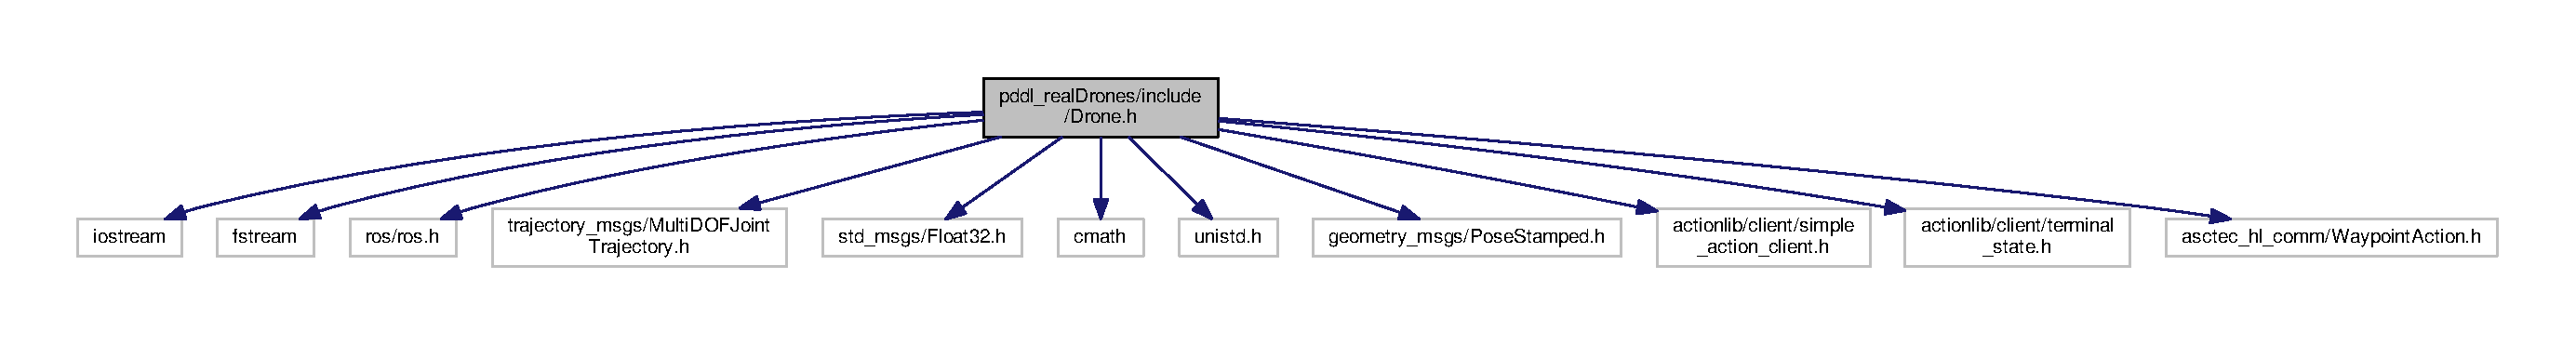
\includegraphics[width=350pt]{pddl__realDrones_2include_2Drone_8h__incl}
\end{center}
\end{figure}
This graph shows which files directly or indirectly include this file\+:\nopagebreak
\begin{figure}[H]
\begin{center}
\leavevmode
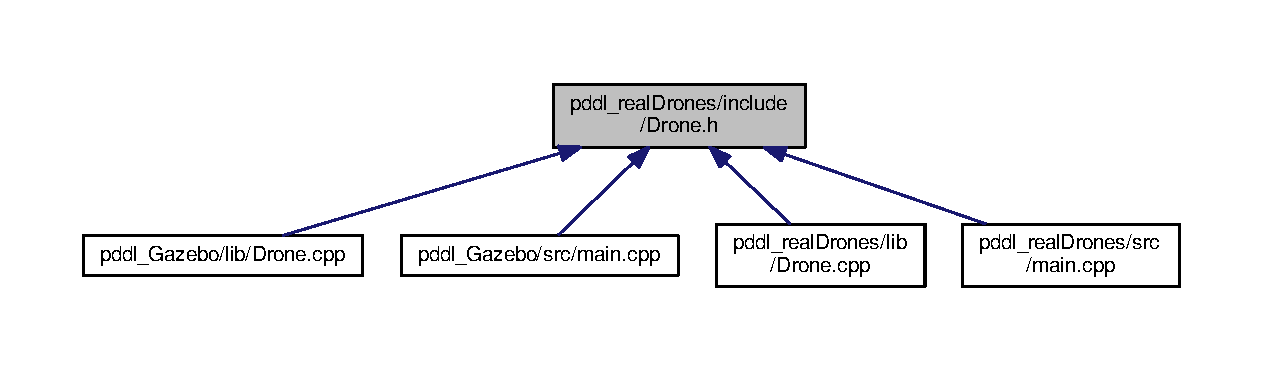
\includegraphics[width=350pt]{pddl__realDrones_2include_2Drone_8h__dep__incl}
\end{center}
\end{figure}
\subsection*{Classes}
\begin{DoxyCompactItemize}
\item 
class \hyperlink{classDrone}{Drone}
\end{DoxyCompactItemize}

\input{pddl__Gazebo_2lib_2Drone_8cpp}
\hypertarget{pddl__realDrones_2lib_2Drone_8cpp}{}\section{pddl\+\_\+real\+Drones/lib/\+Drone.cpp File Reference}
\label{pddl__realDrones_2lib_2Drone_8cpp}\index{pddl\+\_\+real\+Drones/lib/\+Drone.\+cpp@{pddl\+\_\+real\+Drones/lib/\+Drone.\+cpp}}
{\ttfamily \#include \char`\"{}Drone.\+h\char`\"{}}\newline
Include dependency graph for Drone.\+cpp\+:\nopagebreak
\begin{figure}[H]
\begin{center}
\leavevmode
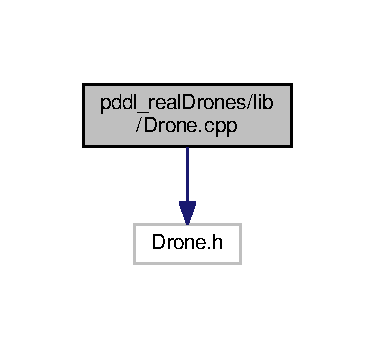
\includegraphics[width=180pt]{pddl__realDrones_2lib_2Drone_8cpp__incl}
\end{center}
\end{figure}
\subsection*{Functions}
\begin{DoxyCompactItemize}
\item 
void \hyperlink{pddl__realDrones_2lib_2Drone_8cpp_a9e24a1a9a80fc7fc15b7f2f9e09f8b86}{feedback\+CB} (const asctec\+\_\+hl\+\_\+comm\+::\+Waypoint\+Feedback\+Const\+Ptr \&fb)
\item 
void \hyperlink{pddl__realDrones_2lib_2Drone_8cpp_a95e6fd6e0fa68d392b633b686f5ea889}{active\+Cb} ()
\item 
void \hyperlink{pddl__realDrones_2lib_2Drone_8cpp_abf245bd90872a8610d5b8a7981fc338f}{done\+Cb} (const actionlib\+::\+Simple\+Client\+Goal\+State \&state, const asctec\+\_\+hl\+\_\+comm\+::\+Waypoint\+Result\+Const\+Ptr \&result)
\end{DoxyCompactItemize}


\subsection{Function Documentation}
\mbox{\Hypertarget{pddl__realDrones_2lib_2Drone_8cpp_a95e6fd6e0fa68d392b633b686f5ea889}\label{pddl__realDrones_2lib_2Drone_8cpp_a95e6fd6e0fa68d392b633b686f5ea889}} 
\index{pddl\+\_\+real\+Drones/lib/\+Drone.\+cpp@{pddl\+\_\+real\+Drones/lib/\+Drone.\+cpp}!active\+Cb@{active\+Cb}}
\index{active\+Cb@{active\+Cb}!pddl\+\_\+real\+Drones/lib/\+Drone.\+cpp@{pddl\+\_\+real\+Drones/lib/\+Drone.\+cpp}}
\subsubsection{\texorpdfstring{active\+Cb()}{activeCb()}}
{\footnotesize\ttfamily void active\+Cb (\begin{DoxyParamCaption}{ }\end{DoxyParamCaption})}


\begin{DoxyCode}
20 \{
21     ROS\_INFO(\textcolor{stringliteral}{"Goal just went active"});
22 \}
\end{DoxyCode}
\mbox{\Hypertarget{pddl__realDrones_2lib_2Drone_8cpp_abf245bd90872a8610d5b8a7981fc338f}\label{pddl__realDrones_2lib_2Drone_8cpp_abf245bd90872a8610d5b8a7981fc338f}} 
\index{pddl\+\_\+real\+Drones/lib/\+Drone.\+cpp@{pddl\+\_\+real\+Drones/lib/\+Drone.\+cpp}!done\+Cb@{done\+Cb}}
\index{done\+Cb@{done\+Cb}!pddl\+\_\+real\+Drones/lib/\+Drone.\+cpp@{pddl\+\_\+real\+Drones/lib/\+Drone.\+cpp}}
\subsubsection{\texorpdfstring{done\+Cb()}{doneCb()}}
{\footnotesize\ttfamily void done\+Cb (\begin{DoxyParamCaption}\item[{const actionlib\+::\+Simple\+Client\+Goal\+State \&}]{state,  }\item[{const asctec\+\_\+hl\+\_\+comm\+::\+Waypoint\+Result\+Const\+Ptr \&}]{result }\end{DoxyParamCaption})}


\begin{DoxyCode}
25 \{
26     \textcolor{keywordflow}{if} (state.state\_ == actionlib::SimpleClientGoalState::SUCCEEDED)
27     \{
28         ROS\_INFO(\textcolor{stringliteral}{"Finished in state [%s]"}, state.toString().c\_str());
29     \}
30     \textcolor{keywordflow}{else}
31     \{
32         ROS\_WARN(\textcolor{stringliteral}{"Finished in state [%s]"}, state.toString().c\_str());
33     \}
34     \textcolor{keyword}{const} geometry\_msgs::Point32 & wp = result->result\_pos;
35     ROS\_INFO(\textcolor{stringliteral}{"Reached waypoint: %fm %fm %fm %f°"},wp.x, wp.y, wp.z, result->result\_yaw*180/M\_PI);
36 \}
\end{DoxyCode}
\mbox{\Hypertarget{pddl__realDrones_2lib_2Drone_8cpp_a9e24a1a9a80fc7fc15b7f2f9e09f8b86}\label{pddl__realDrones_2lib_2Drone_8cpp_a9e24a1a9a80fc7fc15b7f2f9e09f8b86}} 
\index{pddl\+\_\+real\+Drones/lib/\+Drone.\+cpp@{pddl\+\_\+real\+Drones/lib/\+Drone.\+cpp}!feedback\+CB@{feedback\+CB}}
\index{feedback\+CB@{feedback\+CB}!pddl\+\_\+real\+Drones/lib/\+Drone.\+cpp@{pddl\+\_\+real\+Drones/lib/\+Drone.\+cpp}}
\subsubsection{\texorpdfstring{feedback\+C\+B()}{feedbackCB()}}
{\footnotesize\ttfamily void feedback\+CB (\begin{DoxyParamCaption}\item[{const asctec\+\_\+hl\+\_\+comm\+::\+Waypoint\+Feedback\+Const\+Ptr \&}]{fb }\end{DoxyParamCaption})}


\begin{DoxyCode}
14 \{
15     \textcolor{keyword}{const} geometry\_msgs::Point32 & wp = fb->current\_pos;
16     ROS\_INFO(\textcolor{stringliteral}{"got feedback: %fm %fm %fm %f° "}, wp.x, wp.y, wp.z, fb->current\_yaw*180/M\_PI);
17 \}
\end{DoxyCode}

\input{pddl__Gazebo_2src_2main_8cpp}
\hypertarget{pddl__realDrones_2src_2main_8cpp}{}\section{pddl\+\_\+real\+Drones/src/main.cpp File Reference}
\label{pddl__realDrones_2src_2main_8cpp}\index{pddl\+\_\+real\+Drones/src/main.\+cpp@{pddl\+\_\+real\+Drones/src/main.\+cpp}}
{\ttfamily \#include $<$ros/ros.\+h$>$}\newline
{\ttfamily \#include $<$std\+\_\+msgs/\+Float32.\+h$>$}\newline
{\ttfamily \#include $<$cmath$>$}\newline
{\ttfamily \#include $<$unistd.\+h$>$}\newline
{\ttfamily \#include $<$geometry\+\_\+msgs/\+Pose\+Stamped.\+h$>$}\newline
{\ttfamily \#include \char`\"{}Drone.\+h\char`\"{}}\newline
{\ttfamily \#include $<$iostream$>$}\newline
{\ttfamily \#include $<$fstream$>$}\newline
Include dependency graph for main.\+cpp\+:\nopagebreak
\begin{figure}[H]
\begin{center}
\leavevmode
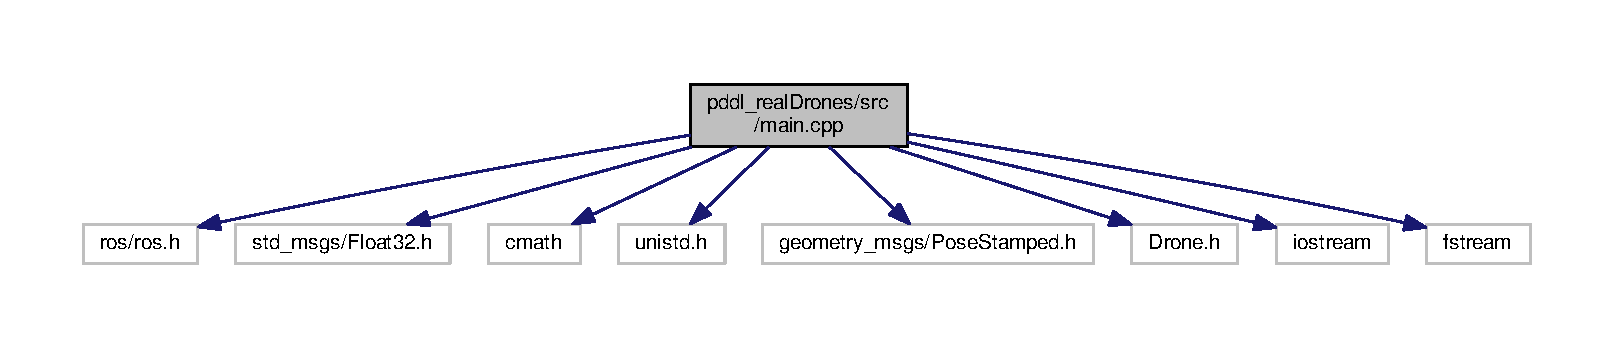
\includegraphics[width=350pt]{pddl__realDrones_2src_2main_8cpp__incl}
\end{center}
\end{figure}
\subsection*{Classes}
\begin{DoxyCompactItemize}
\item 
struct \hyperlink{structPoint}{Point}
\end{DoxyCompactItemize}
\subsection*{Macros}
\begin{DoxyCompactItemize}
\item 
\#define \hyperlink{pddl__realDrones_2src_2main_8cpp_a2cd1c8d16c60718e3142175e2a5a7656}{num\+Drones}~1 /$\ast$$\ast$ @def Number of drones piloted $\ast$/
\end{DoxyCompactItemize}
\subsection*{Functions}
\begin{DoxyCompactItemize}
\item 
int \hyperlink{pddl__realDrones_2src_2main_8cpp_a0ddf1224851353fc92bfbff6f499fa97}{main} (int argc, char $\ast$argv\mbox{[}$\,$\mbox{]})
\end{DoxyCompactItemize}


\subsection{Macro Definition Documentation}
\mbox{\Hypertarget{pddl__realDrones_2src_2main_8cpp_a2cd1c8d16c60718e3142175e2a5a7656}\label{pddl__realDrones_2src_2main_8cpp_a2cd1c8d16c60718e3142175e2a5a7656}} 
\index{pddl\+\_\+real\+Drones/src/main.\+cpp@{pddl\+\_\+real\+Drones/src/main.\+cpp}!num\+Drones@{num\+Drones}}
\index{num\+Drones@{num\+Drones}!pddl\+\_\+real\+Drones/src/main.\+cpp@{pddl\+\_\+real\+Drones/src/main.\+cpp}}
\subsubsection{\texorpdfstring{num\+Drones}{numDrones}}
{\footnotesize\ttfamily \#define num\+Drones~1 /$\ast$$\ast$ @def Number of drones piloted $\ast$/}



\subsection{Function Documentation}
\mbox{\Hypertarget{pddl__realDrones_2src_2main_8cpp_a0ddf1224851353fc92bfbff6f499fa97}\label{pddl__realDrones_2src_2main_8cpp_a0ddf1224851353fc92bfbff6f499fa97}} 
\index{pddl\+\_\+real\+Drones/src/main.\+cpp@{pddl\+\_\+real\+Drones/src/main.\+cpp}!main@{main}}
\index{main@{main}!pddl\+\_\+real\+Drones/src/main.\+cpp@{pddl\+\_\+real\+Drones/src/main.\+cpp}}
\subsubsection{\texorpdfstring{main()}{main()}}
{\footnotesize\ttfamily int main (\begin{DoxyParamCaption}\item[{int}]{argc,  }\item[{char $\ast$}]{argv\mbox{[}$\,$\mbox{]} }\end{DoxyParamCaption})}

$<$ first position of each drone

Initialisation of the drones

Initialisation of the map Counting the number of points

Creating each point of the map

Reading the plan

Positioning each drone to its first position

Sending the position read from the plan 
\begin{DoxyCode}
31 \{
32    
33     \hyperlink{structPoint}{Point} *point;
34     std::string node;
35     std::string action;
36     std::string name;
37     std::string movefrom;
38     std::string moveto;
39     \textcolor{keywordtype}{bool} check=0;
40     \textcolor{keywordtype}{double} xmove;
41     \textcolor{keywordtype}{double} ymove;
42     \textcolor{keywordtype}{double} zmove;
43     \textcolor{keywordtype}{int} i=0;
44     \textcolor{keywordtype}{int} k=0; 
45     \textcolor{keywordtype}{int} position [\hyperlink{pddl__realDrones_2src_2main_8cpp_a2cd1c8d16c60718e3142175e2a5a7656}{numDrones}]=\{20\textcolor{comment}{/*, 315, 512*/}\}; 
46     \textcolor{keywordtype}{int} move=0;
47     \hyperlink{classDrone}{Drone} drones [\hyperlink{pddl__realDrones_2src_2main_8cpp_a2cd1c8d16c60718e3142175e2a5a7656}{numDrones}];
48     ros::init (argc, argv, \textcolor{stringliteral}{"pddl"});
49     ros::NodeHandle nh;
50     ros::Duration timeout(1);
51 
53     \textcolor{keywordflow}{for} (\textcolor{keywordtype}{int} i=0; i< \hyperlink{pddl__realDrones_2src_2main_8cpp_a2cd1c8d16c60718e3142175e2a5a7656}{numDrones}; i++)
54     \{
55         drones[i].\hyperlink{classDrone_a8598b7ea716264e8428a4963a13252fb}{setDrone}(i, nh);
56     \}
57 
60     \textcolor{comment}{/*TODO use function count line who return k*/}
61     std::ifstream file(\textcolor{stringliteral}{"/home/carabidouil/catkin\_ws/src/pddl/plan/map\_coordinates.pddl"}, std::ios\_base::in)
      ;
62     \textcolor{keywordflow}{if} (file.is\_open()) 
63     \{
64     \textcolor{keywordflow}{while} (std::getline(file, node))
65     \{
66             k++;
67     \}
68             file.close();
69     \}
70     \textcolor{keywordflow}{else} 
71     \{
72         std::cout << \textcolor{stringliteral}{"Error opening file map\_coordinates\(\backslash\)n"};
73     \}
74 
76     point = \textcolor{keyword}{new} \hyperlink{structPoint}{Point}[k];
77     std::ifstream myfile(\textcolor{stringliteral}{"/home/carabidouil/catkin\_ws/src/pddl/plan/map\_coordinates.pddl"}, 
      std::ios\_base::in);   
78     \textcolor{keywordflow}{if} (myfile.is\_open()) 
79     \{
80         \textcolor{keywordflow}{while} (myfile >> node >>xmove >> ymove>>zmove )
81         \{
82         point[i].\hyperlink{structPoint_a0f88d21a7c21079e24a66fa177b62d58}{node}=node;
83             point[i].\hyperlink{structPoint_ab99c56589bc8ad5fa5071387110a5bc7}{x}=xmove;
84             point[i].\hyperlink{structPoint_afa38be143ae800e6ad69ce8ed4df62d8}{y}=ymove;
85             point[i].\hyperlink{structPoint_a05ba3b1dfcb19430582ae953cbbfbded}{z}=zmove;
86             i++;   
87     \}
88         std::cout << \textcolor{stringliteral}{"the map is set."}<<std::endl;
89     myfile.close() ; 
90     \}
91     \textcolor{keywordflow}{else} 
92     \{
93         std::cout << \textcolor{stringliteral}{"Error opening file map\_coordinates\(\backslash\)n"};
94     \}
95     
97     std::ifstream pfile(\textcolor{stringliteral}{"/home/carabidouil/catkin\_ws/src/pddl/plan/plan.pddl"}, std::ios\_base::in);     
98     \textcolor{keywordflow}{if} (pfile.is\_open()) 
99     \{
101     std::cout<<\textcolor{stringliteral}{"Positioning the drones."}<<std::endl;
102     \textcolor{keywordflow}{for} (\textcolor{keywordtype}{int} i=0; i<\hyperlink{pddl__realDrones_2src_2main_8cpp_a2cd1c8d16c60718e3142175e2a5a7656}{numDrones}; i++)
103     \{
104         \textcolor{keywordflow}{while}(!check)
105         \{
106             ros::spinOnce();
107             check=drones[i].\hyperlink{classDrone_a106284f63c05f3f112435b2cb5c4896c}{move}(point[position[i]].x, point[position[i]].y, point[position[i]].z);
108             sleep(15);
109         \}
110         check=0;    
111         \}
112     std::cout<< \textcolor{stringliteral}{"All drones are positioned."}<<std::endl;
113     \textcolor{keywordtype}{int} l=0;
115         \textcolor{keywordflow}{while} (ros::ok())
116     \{
117         \textcolor{keywordflow}{while} (pfile >> action >>name >> movefrom>>moveto )
118         \{
119             std::cout <<\textcolor{stringliteral}{"Next action is read."}<<std::endl;
120             \textcolor{keywordtype}{int} position =0;
121             \textcolor{keywordflow}{while}(moveto!=point[position].node)position++; 
122             \textcolor{keywordflow}{for} (\textcolor{keywordtype}{int} i=0; i<\hyperlink{pddl__realDrones_2src_2main_8cpp_a2cd1c8d16c60718e3142175e2a5a7656}{numDrones}; i++)
123             \{
124                 \textcolor{keywordflow}{if} (drones[i].getName()==name)
125                 \{
126                     \textcolor{keywordflow}{while}(!check)
127                     \{
128                         std::cout << \textcolor{stringliteral}{"the drone "} <<i<< \textcolor{stringliteral}{"is asked to move to "}<<position<<std::endl;
129                         ros::spinOnce();
130                         check=drones[i].\hyperlink{classDrone_a106284f63c05f3f112435b2cb5c4896c}{move}(point[position].x, point[position].y, point[position].z);
131                         sleep(5);
132                     \}
133                     check=0;
134                 \}
135             \}
136         \}   
137     \}
138     \}
139     \textcolor{keywordflow}{else} 
140     \{
141         std::cout << \textcolor{stringliteral}{"Error opening file plan\(\backslash\)n"};
142     \}
143     getchar();
144     \textcolor{keywordflow}{return} 0;
145 
146 \}
\end{DoxyCode}

\hypertarget{build__problem_8c}{}\section{Sof\+A\+R/build\+\_\+problem.c File Reference}
\label{build__problem_8c}\index{Sof\+A\+R/build\+\_\+problem.\+c@{Sof\+A\+R/build\+\_\+problem.\+c}}


script that builds the map and the problem for the pddl plan  


{\ttfamily \#include $<$stdlib.\+h$>$}\newline
{\ttfamily \#include $<$stdio.\+h$>$}\newline
{\ttfamily \#include $<$string.\+h$>$}\newline
{\ttfamily \#include $<$math.\+h$>$}\newline
Include dependency graph for build\+\_\+problem.\+c\+:\nopagebreak
\begin{figure}[H]
\begin{center}
\leavevmode
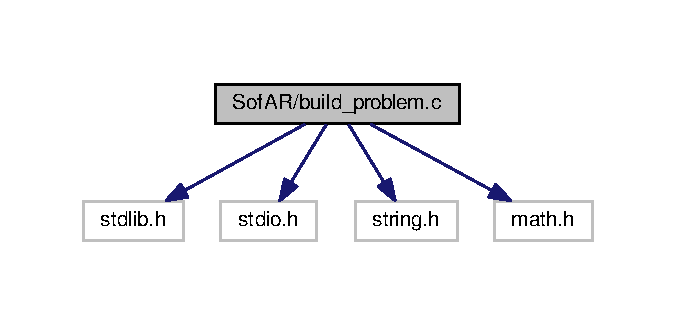
\includegraphics[width=325pt]{build__problem_8c__incl}
\end{center}
\end{figure}
\subsection*{Functions}
\begin{DoxyCompactItemize}
\item 
int \hyperlink{build__problem_8c_a840291bc02cba5474a4cb46a9b9566fe}{main} (void)
\end{DoxyCompactItemize}


\subsection{Detailed Description}
script that builds the map and the problem for the pddl plan 

Enrico B\+O\+R\+E\+L\+LO (\href{mailto:enrico.borello@yahoo.it}{\tt enrico.\+borello@yahoo.\+it})  Louise B\+R\+A\+S\+S\+E\+UR (\href{mailto:louise.brasseur@etu.utc.fr}{\tt louise.\+brasseur@etu.\+utc.\+fr}) \begin{DoxyDate}{Date}
March, 2017 This script takes into account the parameters of the problem and creates the map and the problem files with the pddl format. 
\end{DoxyDate}


\subsection{Function Documentation}
\mbox{\Hypertarget{build__problem_8c_a840291bc02cba5474a4cb46a9b9566fe}\label{build__problem_8c_a840291bc02cba5474a4cb46a9b9566fe}} 
\index{build\+\_\+problem.\+c@{build\+\_\+problem.\+c}!main@{main}}
\index{main@{main}!build\+\_\+problem.\+c@{build\+\_\+problem.\+c}}
\subsubsection{\texorpdfstring{main()}{main()}}
{\footnotesize\ttfamily int main (\begin{DoxyParamCaption}\item[{void}]{ }\end{DoxyParamCaption})}


\begin{DoxyCode}
17 \{
18     \textcolor{keywordtype}{float} globalLength, globalWidth, globalDepth;
19     \textcolor{keywordtype}{float} X, Y, Z;
20     \textcolor{keywordtype}{int} width, length, depth;
21     \textcolor{keywordtype}{float} minSize;
22     \textcolor{keywordtype}{int} drones;
23     \textcolor{keywordtype}{int} area;
24     \textcolor{keywordtype}{int} empty;
25     \textcolor{comment}{//getting the parameters of the problem}
26     printf(\textcolor{stringliteral}{"What is the width of your map in meters : "});
27     scanf (\textcolor{stringliteral}{"%f"},&globalWidth);
28     printf(\textcolor{stringliteral}{"What is the length of your map in meters : "});
29     scanf (\textcolor{stringliteral}{"%f"},&globalLength);
30     printf(\textcolor{stringliteral}{"What is the depth of your map in meters : "});
31     scanf (\textcolor{stringliteral}{"%f"},&globalDepth);
32     printf(\textcolor{stringliteral}{"What is the diameter of the biggest drone in meter : "});
33     scanf (\textcolor{stringliteral}{"%f"},&minSize);
34     printf(\textcolor{stringliteral}{"How many drones do you want on the map : "});
35     scanf (\textcolor{stringliteral}{"%d"},&drones);
36     width=floor(globalWidth/minSize);
37     length=floor(globalLength/minSize);
38     globalDepth = globalDepth-0.5;
39     depth=floor(globalDepth/0.3);
40     \textcolor{keywordtype}{int} start[drones];
41     \textcolor{keywordtype}{int} stop[drones];
42     \textcolor{comment}{//getting the starting and final point for each drone}
43     \textcolor{keywordflow}{for} (\textcolor{keywordtype}{int} i=0; i<drones; i++)
44     \{
45         \textcolor{keywordflow}{do} \{
46             printf(\textcolor{stringliteral}{"Where should drone %i start : "}, i);
47             \textcolor{keywordflow}{do} \{
48                 printf(\textcolor{stringliteral}{"X : "});
49                 scanf (\textcolor{stringliteral}{"%f"},&X);
50             \} \textcolor{keywordflow}{while} (fabs(X) >= globalWidth/2);
51             \textcolor{keywordflow}{do} \{
52                 printf(\textcolor{stringliteral}{"Y : "});
53                 scanf (\textcolor{stringliteral}{"%f"},&Y);
54             \} \textcolor{keywordflow}{while} (fabs(Y) >= globalLength/2);
55             \textcolor{keywordflow}{do} \{
56                 printf(\textcolor{stringliteral}{"Z : "});
57                 scanf (\textcolor{stringliteral}{"%f"},&Z);
58             \} \textcolor{keywordflow}{while} (Z >= globalDepth+0.5 || Z < 0.5);
59             Z=floor((Z-0.5)/0.3);
60             Y=floor((Y+globalLength/2)/(globalLength/length));
61             X=floor((X+globalWidth/2)/(globalWidth/width));
62             start[i] = Z+(Y+X*length)*depth;
63             empty=0;
64             \textcolor{keywordflow}{for} (\textcolor{keywordtype}{int} j=0; j<i; j++)
65             \{
66                 \textcolor{keywordflow}{if} (start[i]==start[j]) empty++;
67             \}
68         \} \textcolor{keywordflow}{while} (start[i]<0 || start[i]>=length*width*depth || empty!=0);
69         \textcolor{keywordflow}{do} \{
70             printf(\textcolor{stringliteral}{"Where should drone %i stop : "}, i);
71             \textcolor{keywordflow}{do} \{
72                 printf(\textcolor{stringliteral}{"X : "});
73                 scanf (\textcolor{stringliteral}{"%f"},&X);
74             \} \textcolor{keywordflow}{while} (fabs(X) >= globalWidth/2);
75             \textcolor{keywordflow}{do} \{
76                 printf(\textcolor{stringliteral}{"Y : "});
77                 scanf (\textcolor{stringliteral}{"%f"},&Y);
78             \} \textcolor{keywordflow}{while} (fabs(Y) >= globalLength/2);
79             \textcolor{keywordflow}{do} \{
80                 printf(\textcolor{stringliteral}{"Z : "});
81                 scanf (\textcolor{stringliteral}{"%f"},&Z);
82             \} \textcolor{keywordflow}{while} (Z >= globalDepth+0.5 || Z < 0.5);
83             Z=floor((Z-0.5)/0.3);
84             Y=floor((Y+globalLength/2)/(globalLength/length));
85             X=floor((X+globalWidth/2)/(globalWidth/width));
86             stop[i] = Z+(Y+X*length)*depth;
87             empty=0;
88             \textcolor{keywordflow}{for} (\textcolor{keywordtype}{int} j=0; j<i; j++)
89             \{
90                 \textcolor{keywordflow}{if} (stop[i]==stop[j]) empty++;
91             \}
92         \} \textcolor{keywordflow}{while} (stop[i]<0 || stop[i]>=length*width*depth || empty!=0);
93         
94     \}
95 
96     \textcolor{comment}{//Writting the problem and map\_coordinates files}
97     FILE *myPlanFile;
98     FILE *myMapFile;
99     myPlanFile = fopen(\textcolor{stringliteral}{"script\_problem\_test.pddl"}, \textcolor{stringliteral}{"w"});
100     myMapFile = fopen(\textcolor{stringliteral}{"map\_coordinates.pddl"}, \textcolor{stringliteral}{"w"});
101     \textcolor{keywordflow}{if} (myPlanFile!=NULL && myMapFile!=NULL)
102     \{
103         fprintf(myPlanFile,\textcolor{stringliteral}{"(define\(\backslash\)n\(\backslash\)t(problem script\_problem\_test )\(\backslash\)n\(\backslash\)t(:domain SofAR)\(\backslash\)n\(\backslash\)t(:objects"});
104         \textcolor{keywordflow}{for} (\textcolor{keywordtype}{int} i=0; i<drones; i++)
105         \{
106             fprintf(myPlanFile, \textcolor{stringliteral}{"\(\backslash\)n\(\backslash\)t\(\backslash\)tdrone%i - drone"}, i);
107         \}
108         \textcolor{comment}{//defining the areas}
109         \textcolor{keywordflow}{for} (\textcolor{keywordtype}{int} i=0; i<width; i++)
110         \{
111             \textcolor{keywordflow}{for} (\textcolor{keywordtype}{int} j=0; j<length; j++)
112             \{
113                 \textcolor{keywordflow}{for} (\textcolor{keywordtype}{int} k=0; k<depth; k++)
114                 \{
115                     area = k+(j+i*length)*depth;
116                     fprintf(myPlanFile, \textcolor{stringliteral}{"\(\backslash\)n\(\backslash\)t\(\backslash\)tarea%i - location"}, area);
117                     fprintf(myMapFile, \textcolor{stringliteral}{"area%i\(\backslash\)t%f\(\backslash\)t%f\(\backslash\)t%f\(\backslash\)n"}, area, i*globalWidth/width-globalWidth/2+
      globalWidth/width/2, j*globalLength/length-globalLength/2+globalLength/length/2, k*0.3+0.5);
118                     
119                 \}
120             \}
121         \}
122         \textcolor{comment}{//starting area of each drone}
123         fprintf(myPlanFile,\textcolor{stringliteral}{"\(\backslash\)n\(\backslash\)t)\(\backslash\)n\(\backslash\)t(:init"});
124         \textcolor{keywordflow}{for} (\textcolor{keywordtype}{int} i=0; i<drones; i++)
125         \{
126             fprintf(myPlanFile,\textcolor{stringliteral}{"\(\backslash\)n\(\backslash\)t\(\backslash\)t(is-in drone%i area%i)"},i, start[i]); 
127         \}
128         \textcolor{comment}{//initialising all areas except the ones where the drones are}
129         \textcolor{keywordflow}{for} (\textcolor{keywordtype}{int} i=0; i<width; i++)
130         \{
131             \textcolor{keywordflow}{for} (\textcolor{keywordtype}{int} j=0; j<length; j++)
132             \{
133                 \textcolor{keywordflow}{for} (\textcolor{keywordtype}{int} k=0; k<depth; k++)
134                 \{
135                     area=k+(j+i*length)*depth;
136                     empty=0;
137                     \textcolor{keywordflow}{for} (\textcolor{keywordtype}{int} l=0; l<drones; l++)
138                     \{
139                         \textcolor{keywordflow}{if} (area==start[l]) empty ++;
140                     \}
141                     \textcolor{keywordflow}{if} (empty==0) fprintf(myPlanFile,\textcolor{stringliteral}{"\(\backslash\)n\(\backslash\)t\(\backslash\)t(is-free area%i)"}, area);
142                 \}
143             \}
144         \}
145         \textcolor{comment}{//conecting each area to the adjacent ones}
146         \textcolor{keywordflow}{for} (\textcolor{keywordtype}{int} i=0; i<width; i++)
147         \{
148             \textcolor{keywordflow}{for} (\textcolor{keywordtype}{int} j=0; j<length; j++)
149             \{
150                 \textcolor{keywordflow}{for} (\textcolor{keywordtype}{int} k=0; k<depth; k++)
151                 \{
152                     area = k+(j+i*length)*depth;
153                     \textcolor{keywordflow}{if} (k-1>=0) fprintf(myPlanFile,\textcolor{stringliteral}{"\(\backslash\)n\(\backslash\)t\(\backslash\)t(connected area%i area%i)"}, area, k-1+(j+i*length
      )*depth);
154                     \textcolor{keywordflow}{if} (k+1<depth) fprintf(myPlanFile,\textcolor{stringliteral}{"\(\backslash\)n\(\backslash\)t\(\backslash\)t(connected area%i area%i)"}, area, k+1+(j+i*
      length)*depth);
155                     \textcolor{keywordflow}{if} (j-1>=0) fprintf(myPlanFile,\textcolor{stringliteral}{"\(\backslash\)n\(\backslash\)t\(\backslash\)t(connected area%i area%i)"}, area, k+((j-1)+i*
      width)*depth);
156                     \textcolor{keywordflow}{if} (j+1<length) fprintf(myPlanFile,\textcolor{stringliteral}{"\(\backslash\)n\(\backslash\)t\(\backslash\)t(connected area%i area%i)"}, area, k+((j+1)+i*
      length)*depth);
157                     \textcolor{keywordflow}{if} (i-1>=0) fprintf(myPlanFile,\textcolor{stringliteral}{"\(\backslash\)n\(\backslash\)t\(\backslash\)t(connected area%i area%i)"}, area, k+(j+(i-1)*
      length)*depth);
158                     \textcolor{keywordflow}{if} (i+1<length) fprintf(myPlanFile,\textcolor{stringliteral}{"\(\backslash\)n\(\backslash\)t\(\backslash\)t(connected area%i area%i)"}, area, k+(j+(i+1)*
      length)*depth);
159                 \}
160             \}
161         \}
162         \textcolor{comment}{//final state of the problem}
163         fprintf(myPlanFile,\textcolor{stringliteral}{"\(\backslash\)n\(\backslash\)t)\(\backslash\)n\(\backslash\)t(:goal (and "});
164         \textcolor{keywordflow}{for} (\textcolor{keywordtype}{int} i=0; i<drones; i++)
165         \{
166             fprintf(myPlanFile,\textcolor{stringliteral}{"(is-in drone%i area%i) (not(is-in drone%i area%i)) "} ,i, stop[i], i, start[
      i] );
167         \}
168         fprintf(myPlanFile,\textcolor{stringliteral}{"))\(\backslash\)n) "});
169 
170         fclose(myPlanFile);
171         fclose(myMapFile);
172     \}
173 \}
\end{DoxyCode}

%--- End generated contents ---

% Index
\backmatter
\newpage
\phantomsection
\clearemptydoublepage
\addcontentsline{toc}{chapter}{Index}
\printindex

\end{document}
